\documentclass[journal,twoside,web]{ieeecolor}
\usepackage{generic}
\usepackage{cite}
\usepackage{amsmath,amssymb,amsfonts}
\usepackage{graphicx}
\usepackage{hyperref}
\hypersetup{hidelinks}
\usepackage{textcomp}
\graphicspath{{fig/}{./}}
\def\BibTeX{{\rm B\kern-.05em{\sc i\kern-.025em b}\kern-.08em
    T\kern-.1667em\lower.7ex\hbox{E}\kern-.125emX}}

\markboth{\hskip20pc IEEE JOURNAL OF INDOOR AND SEAMLESS POSITIONING AND NAVIGATION}
{Xiao: AutoPos: Reference-Free 3D UWB Anchor Self-Calibration from Inter-Anchor Ranging Alone}

\begin{document}

\title{AutoPos: Reference-Free 3D UWB Anchor Self-Calibration from Inter-Anchor Ranging Alone}

\author{Zekai~Xiao}

\maketitle

\begin{abstract}
Deploying an ultra-wideband (UWB) localization system still requires anchor coordinates, a coordinate frame, and residual delay calibration. AutoPos addresses this deployment step with a reference-free 3D anchor self-calibration pipeline for a commodity UWB array. The pipeline estimates a two-layer anchor layout from inter-anchor two-way ranging alone; Vicon, SLAM, total-station survey, and manual anchor measurements are excluded from the calibration loop. AutoPos combines an eight-anchor 4+4 geometry, joint layout and endpoint-delay estimation, and ground-truth-free diagnostics for solution selection. Vicon is used only after calibration to score the recovered layout and the resulting tag coordinates. In an Erlangen laboratory deployment with DWM1001C-class hardware, the production v4-io/T4/F0 pipeline obtains a rigidly registered anchor-layout median residual of 92.8 mm. Over 24 static tag positions, the same layout gives 72.7 mm median 3D localization error, 171.5 mm P95 error, and 109.8 mm RMSE; the median horizontal and vertical errors are 37.4 mm and 61.9 mm, respectively. The full array is observed in 92.2\% of frames, and at least seven anchors are observed in 99.9\% of frames. A deployment-specific Fisher analysis explains why the balanced 4+4 layout is necessary: it changes the vertical self-calibration problem from singular or weakly conditioned to usable, while residual delay--layout coupling remains the main systematic limitation.
\end{abstract}

\begin{IEEEkeywords}
Anchor self-calibration, auto-positioning, indoor positioning, two-way ranging, ultra-wideband, UWB, vertical observability.
\end{IEEEkeywords}

\section{Introduction}
\label{sec:introduction}

\IEEEPARstart{U}{ltra-wideband} (UWB) localization is attractive for indoor motion capture, robotics, sport sensing, and wearable sensing because time-of-flight ranges can be measured with low latency and moderate infrastructure cost. In practice, a deployment is often limited by calibration rather than by the nominal ranging specification. The solver needs anchor coordinates, a coordinate frame, and residual antenna-delay or device-bias terms that are consistent with that frame. Hand measurement, optical survey, and external simultaneous localization and mapping (SLAM) can provide those quantities, but they make the UWB installation dependent on external infrastructure.

AutoPos targets the case in which the anchors are already installed, the anchors can range to one another, and the UWB system must infer its own 3D geometry before tags can be localized. Temporary laboratories, clinics, sport spaces, and field test areas often have this form: the anchor rig is rebuilt or moved, and a full optical survey is not a realistic part of every setup. The benchmark is the accuracy of a coordinate frame calibrated only from inter-anchor UWB ranges and later checked against optical ground truth.

The evaluated system uses eight commodity UWB anchors in a balanced two-layer arrangement, with four lower anchors and four upper anchors. The anchor solver estimates 3D coordinates and per-anchor endpoint-delay terms from the inter-anchor range graph. The tag solver then localizes static tags in the self-calibrated UWB frame. A rigid alignment to Vicon is applied only after calibration so that anchor and tag errors can be expressed in millimetres against an independent reference. Vicon is a validation instrument in this study, not part of the AutoPos calibration method.

The geometry is part of the calibration method. A coplanar UWB anchor layer is singular for vertical anchor perturbations under inter-anchor distances. One raised anchor introduces vertical information but leaves the worst-conditioned lower anchor weakly constrained. The balanced 4+4 layout makes every anchor participate in cross-layer constraints. In the measured geometry, the vertical Fisher bound improves from a mean of about 161 mm with one raised anchor to about 63 mm with four raised anchors, while the worst-anchor bound falls from about 226 mm to about 93 mm. These numbers make the 4+4 array a calibration requirement, not a redundant layout choice.

The paper contributes an evaluated deployment pipeline rather than an isolated range model: reference-free 3D anchor auto-positioning, a measured two-layer observability analysis, and end-to-end Vicon validation on commodity hardware. It reports absolute Vicon-referenced tag error, UWB-internal repeatability, anchor visibility, and ground-truth-free diagnostics. Residual delay--layout coupling remains the main error source and motivates a separate mechanism-focused study.

\section{Related Work}
\label{sec:related}

UWB indoor positioning has been studied with surveyed anchors, inertial sensors, SLAM, and application-specific motion models. UWB and inertial fusion has been used for human movement analysis and lower-body motion capture \cite{kok_2015,zihajehzadeh_2017,yogesh_2023}. These systems show the value of adding independent motion information, but they still require an anchor layout and they address a different operating point from a static, UWB-only, reference-free deployment.

Anchor self-calibration has a separate literature. Batstone et al. formulated time-of-arrival self-calibration using UWB anchors \cite{batstone_2017}, and Corbalan et al. evaluated UWB anchor self-localization in practical settings \cite{corbalan_2023}. Hamer and D'Andrea used a self-calibrating UWB network for multi-robot localization \cite{hamer_2018}, while Ridolfi et al. surveyed and extended self-calibration and collaborative localization techniques for UWB systems \cite{ridolfi_2021}. Multihop and large-scale calibration methods address sparse or extended networks \cite{herbruggen_2023,yuan_2024}. AutoPos is narrower: it tests whether a compact, commodity, two-layer anchor array can generate a useful 3D coordinate system from its own inter-anchor ranges and then localize a tag without an external anchor survey.

Calibration of antenna delay and range bias is closely related. Shah et al. discuss antenna delay calibration of UWB nodes and node calibration for real-time location systems \cite{shah_2021,shah_2022}. Shalaby et al. characterize uncertainty in two-way ranging measurements \cite{shalaby_2023}, and De Preter et al. model range bias and autocalibration in UWB positioning systems \cite{de_preter_2019}. AutoPos uses residual endpoint terms for the same reason: delay and geometry are coupled in a deployed coordinate frame. If the coordinate frame changes, residual corrections must be re-estimated in that frame; otherwise a geometrically accurate anchor layout can still produce poor tag coordinates.

External sensing can resolve coordinate consistency when cameras, maps, or robot trajectories are available. Visual-inertial SLAM aided calibration estimates UWB anchor poses and sensor error parameters \cite{lutz_2019}, and recent coordinate-consistent approaches fuse UWB with SLAM observations \cite{nguyen_2025}. AutoPos removes those inputs from the calibration stage. The new element is the complete deployment path: reference-free 3D anchor layout estimation, a balanced 4+4 vertical geometry, end-to-end Vicon validation, and diagnostics for cases where low UWB residuals do not imply a good positioning frame.

\section{System Model and AutoPos Pipeline}
\label{sec:system}

The deployment contains $N=8$ UWB anchors. Each anchor has an unknown 3D position $\mathbf{x}_i\in\mathbb{R}^3$ and an endpoint correction $b_i$ that captures residual delay and fixed range-bias effects after nominal hardware settings. For an inter-anchor measurement between anchors $i$ and $j$, the fused range is modelled as
\begin{equation}
\hat{d}_{ij} = \lVert \mathbf{x}_i-\mathbf{x}_j\rVert_2 + b_i + b_j + \epsilon_{ij},
\label{eq:range_model}
\end{equation}
where $\epsilon_{ij}$ includes random ranging noise, multipath, and unmodelled residuals. The fitted $b_i$ terms are not bench-measured antenna-delay constants. They are frame-conditioned residual corrections that make the inter-anchor range graph self-consistent for one deployment.

The AutoPos layout solver minimizes robust residuals of (\ref{eq:range_model}) over the anchor coordinates and endpoint corrections, with gauge constraints to remove arbitrary translation and rotation. A regularized endpoint-delay parameterization prevents the layout from explaining all range excess through unconstrained common-mode delay. Without this regularization, geometry and delay variables are weakly separated in a complete but noisy range graph. The production solver version used here is denoted v4-io. It is selected for the static localization pipeline, not for the lowest anchor-only residual under every diagnostic.

After the anchor layout has been estimated, tag localization uses ranges from the tag to the anchors and solves a 3D least-squares position in the AutoPos coordinate frame. For the static evaluation in this paper, each tag position is recorded for 120 s, per-frame UWB positions are computed, and one session-mean coordinate is compared with the corresponding Vicon ground-truth position. The headline tag solver is denoted T4, and the unfiltered output is denoted F0.

Raw AutoPos coordinates have arbitrary orientation and origin, as any range-only layout does. For evaluation, the AutoPos anchor coordinates are rigidly registered to the Vicon anchor coordinates using only anchor correspondences. This rigid alignment has no scale degree of freedom. The same rigid transform is then applied to tag estimates before computing tag error. A Sim(3) similarity fit is reported only as a diagnostic for scale-like layout error; it is not used for headline tag localization.

\section{Two-Layer Geometry and Vertical Observability}
\label{sec:geometry}

The anchor layout uses two vertical layers: four anchors in a lower layer and four anchors in an upper layer. Observability drives this choice. For a single coplanar layer, the derivative of an inter-anchor range with respect to a common out-of-plane displacement is zero at the plane. The vertical part of the self-calibration problem is singular. One raised anchor creates vertical information, but it mostly constrains that raised anchor and leaves lower anchors weakly conditioned. Additional raised anchors distribute vertical constraints across the graph.

\begin{figure}[!t]
\centering
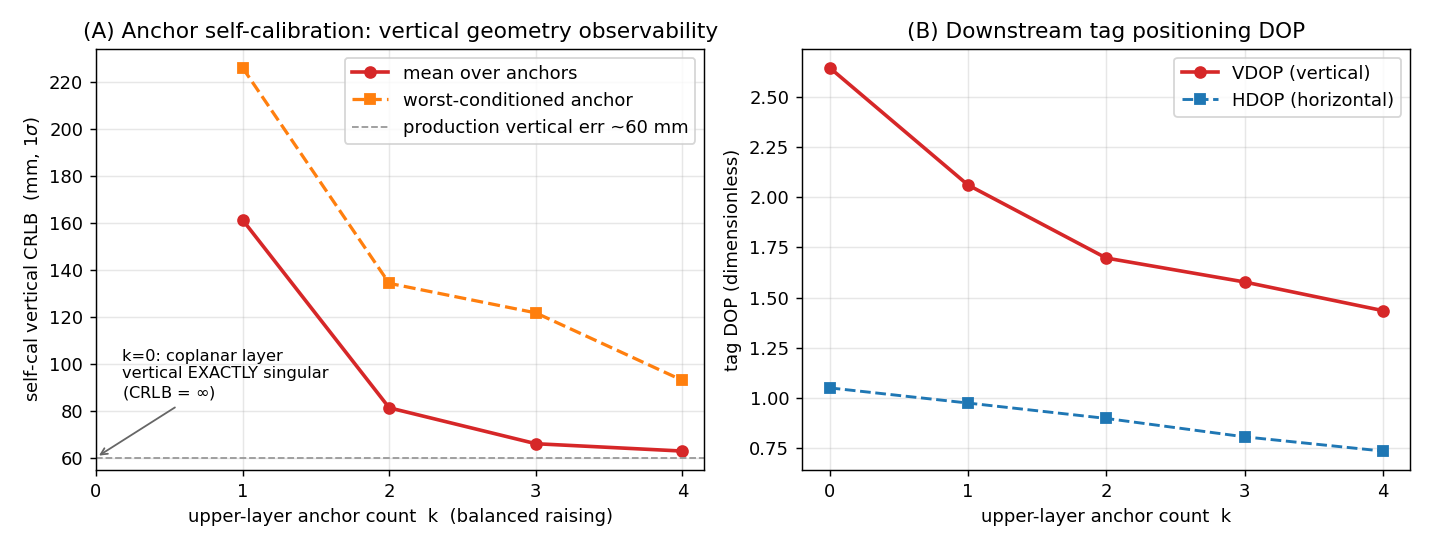
\includegraphics[width=\columnwidth]{vertical_observability_4plus4.png}
\caption{Vertical observability of the two-layer array. A single coplanar layer is singular. Adding raised anchors improves the mean vertical bound, but the worst-anchor bound keeps falling until the balanced 4+4 layout is reached.}
\label{fig:vertical_observability}
\end{figure}

Fig.~\ref{fig:vertical_observability} summarizes the deployment-specific Fisher analysis. With one raised anchor, the mean vertical bound is about 161 mm and the worst-anchor bound is about 226 mm. With two raised anchors, the mean improves to about 81 mm and the worst case to about 134 mm. With three raised anchors, the mean is about 66 mm and the worst case about 122 mm. The balanced 4+4 layout reaches about 63 mm mean vertical bound and about 93 mm worst-anchor bound. The mean bound saturates after two to four raised anchors, but the worst-conditioned anchor continues to improve. That worst-anchor behaviour is the reason the final design uses four upper anchors rather than an asymmetric 4+2 or 4+3 compromise.

The same calculation gives a useful scale for vertical accuracy. The measured median vertical tag error in the static evaluation is 61.9 mm, the same order as the 4+4 vertical bound. This agreement is not a proof of estimator efficiency, because the bound describes anchor self-calibration geometry and the measured value is a tag localization error after the full pipeline. The comparison supports the geometric interpretation of the vertical result rather than attributing it to a favourable post-hoc alignment.

\section{Experimental Setup}
\label{sec:experiment}

The experiment was performed in an Erlangen laboratory using a Vicon motion-capture system as independent ground truth. The UWB system used DWM1001C-class commodity modules arranged as eight anchors and one static tag. The anchor array spans a room-scale volume with four lower anchors and four upper anchors. The evaluated static tag set contains 24 positions distributed across the array footprint, including edge and centre locations, low, middle, and high elevations, and multiple tag-facing directions. Each static position was recorded for approximately 120 s at an intended UWB rate of about 10 Hz.

Vicon was used in two ways. It provided post-hoc ground-truth coordinates for anchors and tags, and it supplied the rigid alignment between the arbitrary AutoPos coordinate gauge and the Vicon frame. Vicon measurements were not used by the AutoPos solver that generated the anchor layout. The input to AutoPos was the recorded inter-anchor UWB range data. This separation keeps the evaluation reference-free at the calibration stage.

Anchor ground truth was computed from Vicon marker data using stable static captures. For each capture, the anchor antenna point was reduced by a coordinate-wise median over frames, and per-capture values were combined across captures. The Vicon camera calibration and marker stability were substantially smaller than the UWB errors reported here, so optical measurement noise is not a plausible explanation for the centimetre-scale UWB residuals. A marker-labelling anomaly affecting anchor G in one dynamic capture was identified during the audit and does not affect the static anchor layout used for headline scoring.

Two metrics are reported for static tags. Vicon-referenced absolute accuracy is the Euclidean error between the session-mean UWB coordinate and the Vicon tag coordinate. UWB-internal repeatability is the frame-to-frame spread of UWB estimates inside the same static session, measured around that session's own UWB cluster. The first metric measures accuracy against an external reference. The second measures stability without Vicon ground truth. Reporting both prevents a stable but biased solution from being mistaken for an accurate one.

\section{Results}
\label{sec:results}

\subsection{Anchor Layout Accuracy}
\label{sec:anchor_results}

Fig.~\ref{fig:layout_overlay} shows the v4-io AutoPos anchor layout after rigid registration to Vicon. The recovered shape is recognizable and metrically useful, but systematic residuals remain after the rigid transform.

\begin{figure}[!t]
\centering
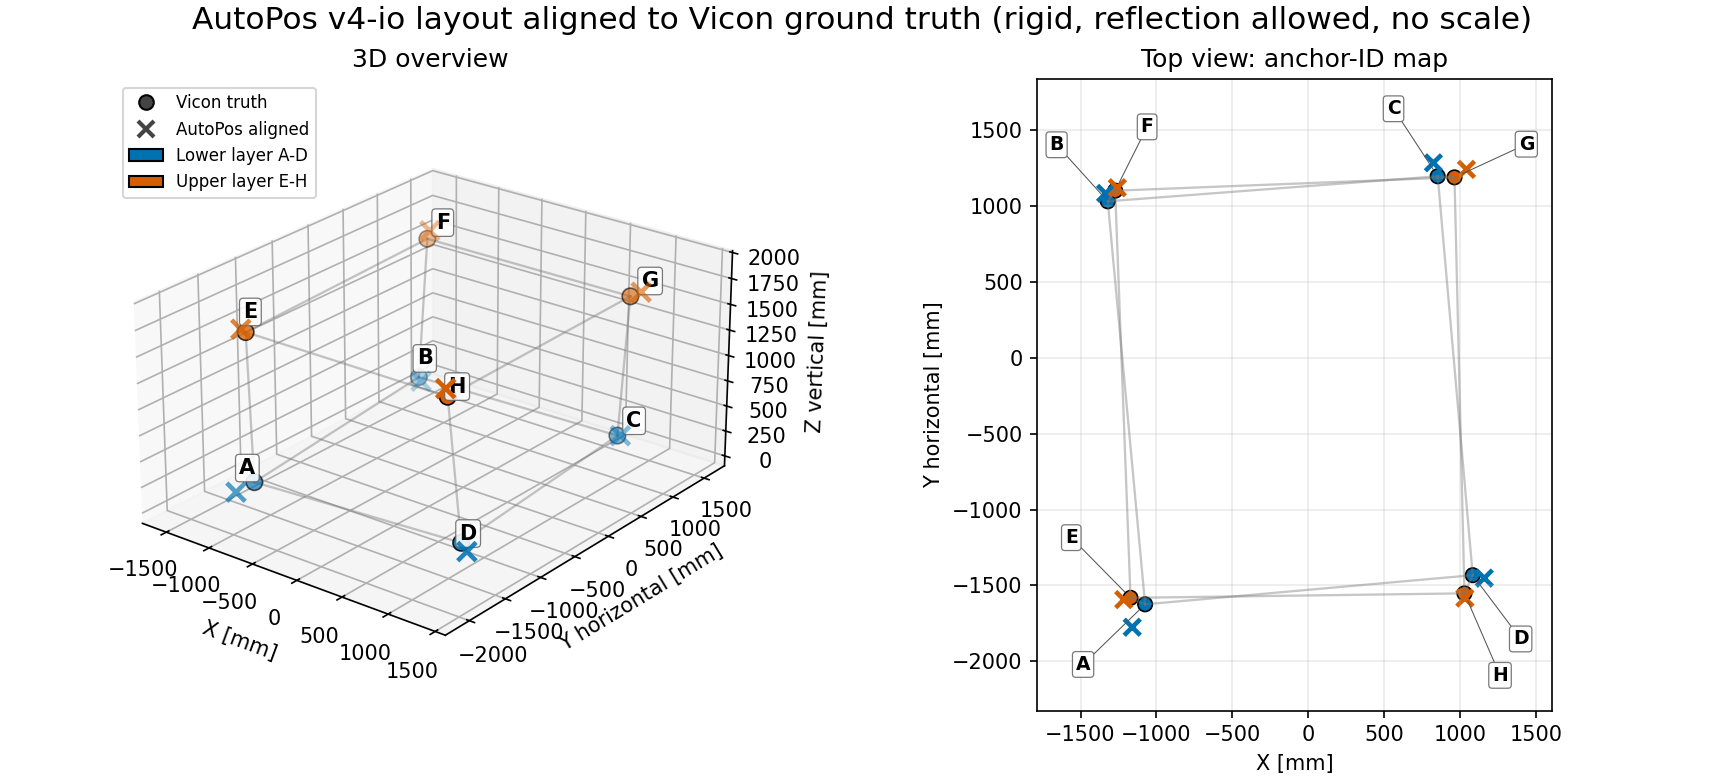
\includegraphics[width=\columnwidth]{autopos_layout_vicon_overlay.png}
\caption{AutoPos v4-io anchor layout after rigid registration to Vicon ground truth. The layout is estimated from inter-anchor UWB ranges alone; Vicon is used only for this post-hoc comparison.}
\label{fig:layout_overlay}
\end{figure}

Table~\ref{tab:anchor_layout} reports the anchor residuals under rigid registration. The production v4-io solver obtains 92.8 mm median residual, 156.9 mm P95 residual, and 105.4 mm RMSE. The horizontal and vertical RMSE components are 86.8 mm and 59.8 mm, respectively. A Sim(3) diagnostic reduces the v4-io layout residual to 67.1 mm, which indicates a coherent scale-like component. The headline result nevertheless uses rigid registration because a deployed range-only layout should not receive an external scale correction after calibration.

\begin{table}[!t]
\caption{Anchor layout residuals after anchor-locked rigid registration to Vicon ground truth.}
\label{tab:anchor_layout}
\centering
\scriptsize
\setlength{\tabcolsep}{3.8pt}
\begin{tabular}{lcccccc}
\hline
Solver & Median & P95 & RMSE & Horiz. RMSE & Vert. RMSE & Sim(3) RMSE\\
 & \multicolumn{3}{c}{3D residual [mm]} & \multicolumn{2}{c}{[mm]} & [mm]\\
\hline
v1-old & 84.6 & 154.1 & 101.3 & 93.8 & 38.1 & 50.1\\
v2 & 127.8 & 184.0 & 136.5 & 109.0 & 82.1 & 60.3\\
v3-lite & 127.9 & 184.2 & 136.6 & 108.8 & 82.6 & 60.9\\
v3-full & 118.9 & 211.7 & 143.4 & 127.5 & 65.8 & 125.3\\
v4-io & 92.8 & 156.9 & 105.4 & 86.8 & 59.8 & 67.1\\
\hline
\end{tabular}
\end{table}

The v1-old solver has the lowest anchor-only RMSE in Table~\ref{tab:anchor_layout}, but anchor residual alone does not predict tag accuracy. The v4-io row gives the best static tag result in the evaluated production pipeline and is used for the headline AutoPos result. In this deployment, the layout that minimizes anchor residuals is not the layout that gives the best tag coordinate frame after residual delays and tag-side effects are included.

\subsection{Static Tag Localization}
\label{sec:static_results}

The headline static result uses the v4-io anchor layout, the T4 tag solver, and unfiltered output. Across 24 static tag positions, one session-mean UWB coordinate is compared with the corresponding Vicon coordinate. The resulting median 3D error is 72.7 mm, with 171.5 mm P95 and 109.8 mm RMSE. The median horizontal error is 37.4 mm and the median vertical error is 61.9 mm.

\begin{table}[!t]
\caption{Static UWB tag localization accuracy for the production v4-io/T4/F0 pipeline. Each row uses one session-mean coordinate for each of 24 static positions.}
\label{tab:static_accuracy}
\centering
\begin{tabular}{lccc}
\hline
Metric & Horizontal [mm] & Vertical [mm] & 3D [mm]\\
\hline
Median error & 37.4 & 61.9 & 72.7\\
P95 error & 73.6 & 170.0 & 171.5\\
RMSE error & 47.9 & 98.8 & 109.8\\
\hline
\end{tabular}
\end{table}

Fig.~\ref{fig:static_cdf} shows the empirical error distribution. The median is sub-decimetre, but the tail remains visible. The P95 error of 171.5 mm is driven mainly by vertical error at difficult positions. Because the static set contains 24 positions, P95 is a descriptive statistic for this campaign rather than a population guarantee. It is reported because it exposes the failure mode hidden by the median.

\begin{figure}[!t]
\centering
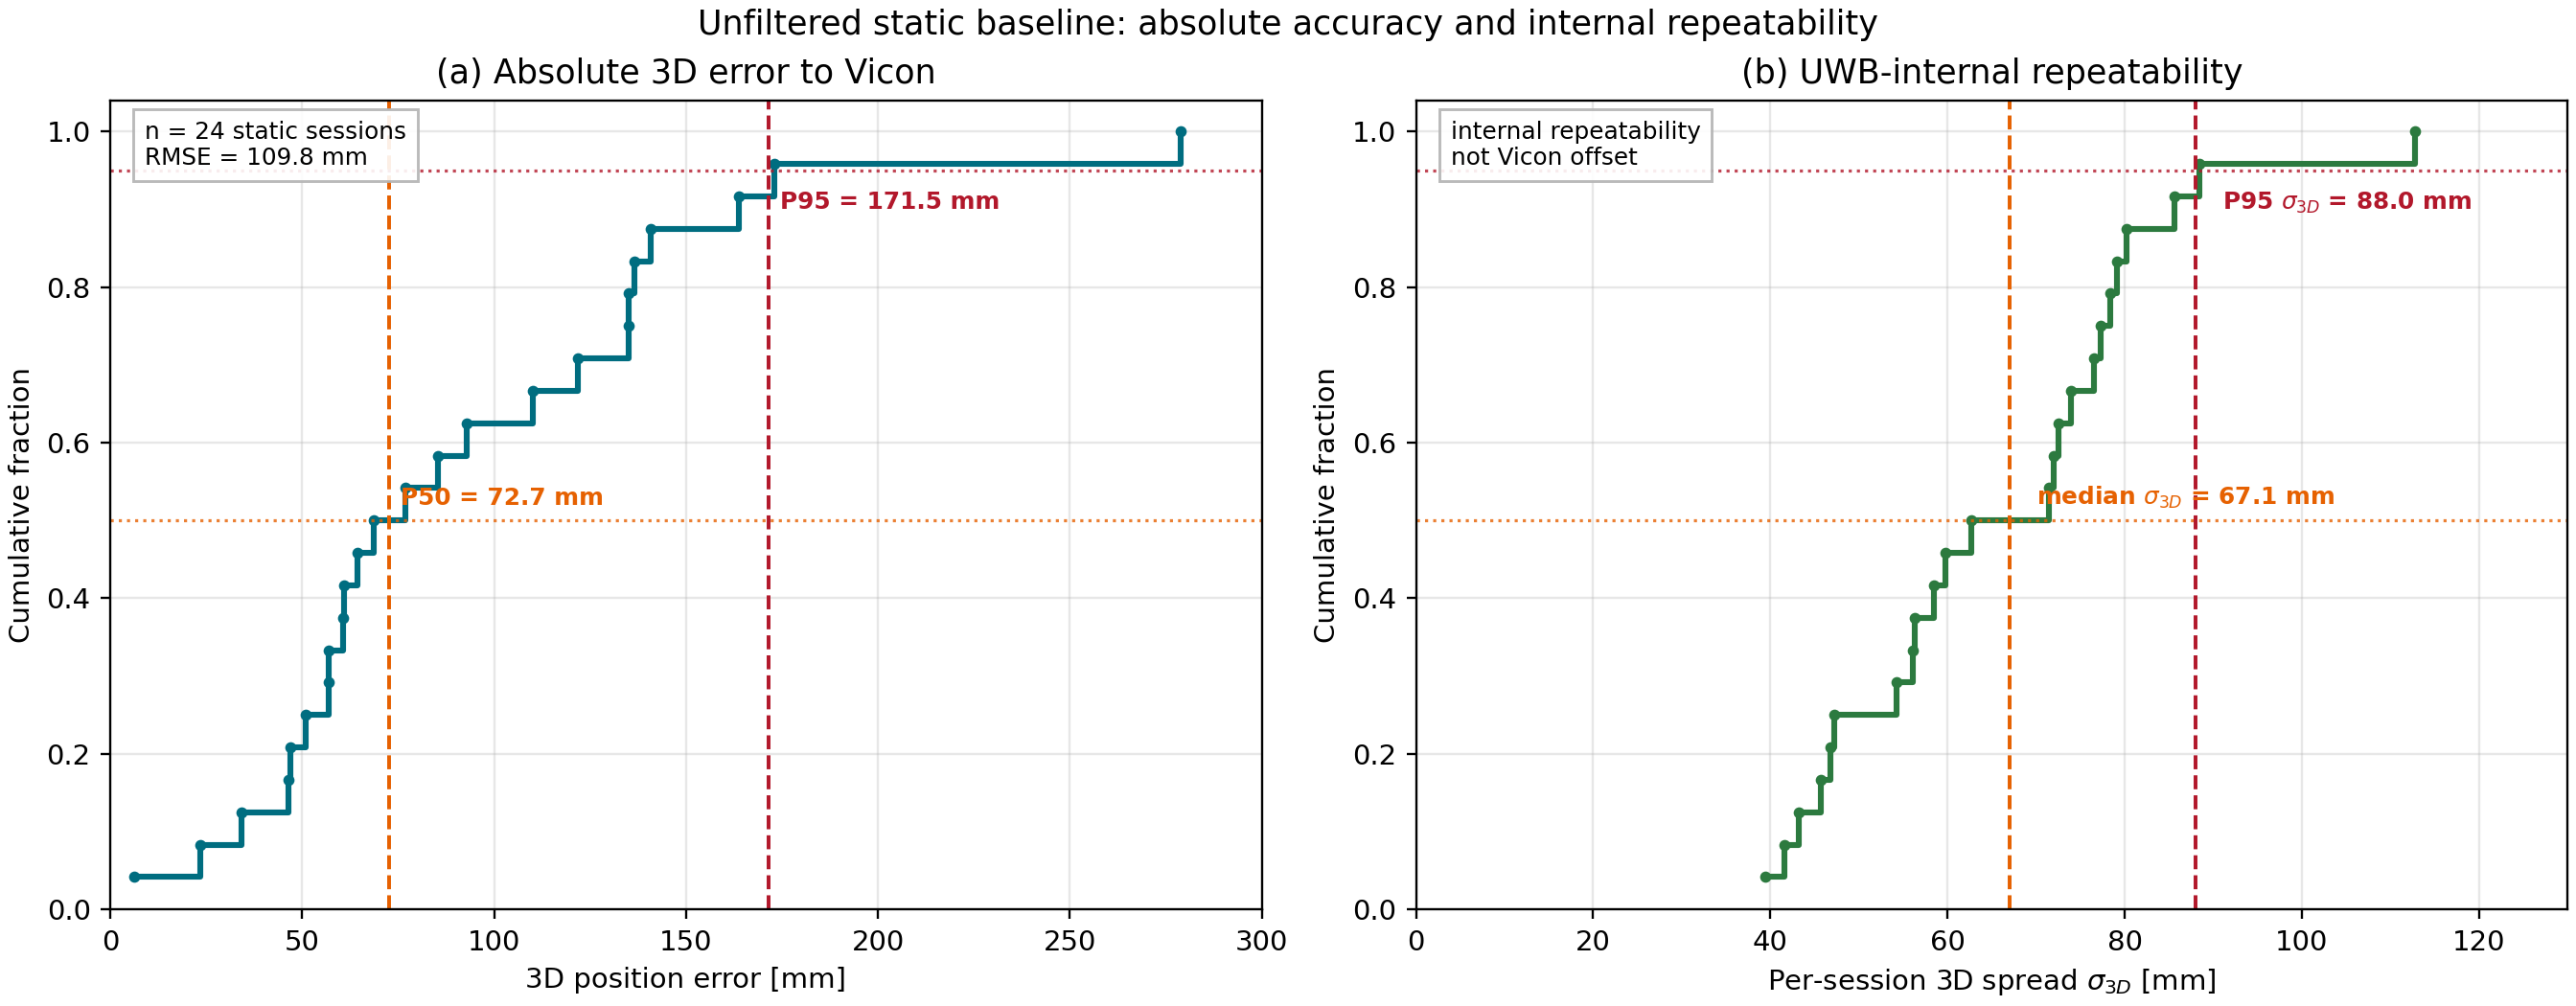
\includegraphics[width=\columnwidth]{static_tag_error_cdf.png}
\caption{Empirical CDF of static tag error for the evaluated AutoPos pipeline. The 3D median is 72.7 mm and the P95 is 171.5 mm over 24 static positions.}
\label{fig:static_cdf}
\end{figure}

Table~\ref{tab:static_sweep} shows the T4 static sweep over the evaluated anchor layouts. The v4-io layout gives the lowest median 3D static error and the lowest horizontal median. Its median internal 3D spread is 67.1 mm, while some alternative layouts have similar or lower spread but worse Vicon-referenced accuracy. Internal stability alone therefore cannot detect coherent coordinate bias.

\begin{table*}[!t]
\caption{Static localization sweep using the common T4 tag solver and session-mean estimator. Absolute accuracy is Vicon-referenced; repeatability is UWB-internal spread within each static session.}
\label{tab:static_sweep}
\centering
\scriptsize
\setlength{\tabcolsep}{3.2pt}
\begin{tabular}{lccccccccccc}
\hline
 & \multicolumn{9}{c}{Vicon-referenced absolute accuracy [mm]} & \multicolumn{2}{c}{UWB-internal repeatability [mm]}\\
Layout & \multicolumn{3}{c}{Median error} & \multicolumn{3}{c}{P95 error} & \multicolumn{3}{c}{RMSE} & Median & P95\\
 & Horiz. & Vert. & 3D & Horiz. & Vert. & 3D & Horiz. & Vert. & 3D & $\sigma_{3D}$ & $\sigma_{3D}$\\
\hline
v1-old & 49.5 & 119.0 & 134.9 & 87.0 & 232.7 & 233.8 & 53.6 & 150.3 & 159.6 & 68.0 & 107.3\\
v2 & 44.1 & 68.3 & 80.9 & 73.2 & 159.9 & 166.8 & 48.7 & 94.2 & 106.1 & 62.7 & 93.2\\
v3-lite & 44.3 & 68.4 & 81.4 & 73.2 & 159.6 & 166.5 & 48.9 & 94.2 & 106.1 & 62.7 & 93.5\\
v3-full & 41.4 & 90.4 & 98.1 & 105.0 & 230.6 & 233.8 & 54.6 & 121.6 & 133.3 & 61.5 & 102.1\\
v4-io & 37.4 & 61.9 & 72.7 & 73.6 & 170.0 & 171.5 & 47.9 & 98.8 & 109.8 & 67.1 & 88.0\\
\hline
\end{tabular}
\end{table*}

\subsection{Anchor Visibility and Redundancy}
\label{sec:visibility}

The 4+4 layout also provides ranging redundancy. Across the 24-position static campaign, 92.2\% of frames ranged to all eight anchors and 99.9\% ranged to at least seven anchors. The link-level success rate was 99.0\%. One anchor contributed most of the missing observations, with about 4.4\% dropout, while the other anchors were below 2\%. The reported static medians are not produced by a rare full-visibility subset. Almost every frame preserves enough cross-layer constraints for the over-determined 3D tag solution.

A two-layer array can only help if both layers are observed. In this experiment, the array was visible enough that the vertical conditioning predicted by the 4+4 geometry is retained in normal static operation. The remaining vertical tail is better explained by systematic bias and residual delay coupling than by frequent loss of upper or lower anchors.

\subsection{Ground-Truth-Free Diagnostics}
\label{sec:diagnostics}

A deployable self-calibration pipeline cannot use Vicon residuals when selecting a layout. It must rely on diagnostics available from the UWB data itself. Simple residual minimization was insufficient in this campaign. In the evaluated solver family, the lowest inter-anchor residual was about 11.5 mm, yet that solution produced one of the worst static positioning outcomes at about 169 mm. The best positioner in the diagnostic comparison had a slightly higher inter-anchor residual of about 12.9 mm while obtaining about 49 mm static 3D median error under its scoring configuration. Low inter-anchor residual is necessary but not sufficient for a good positioning coordinate frame.

More useful diagnostics test stability under anchor subsets and expose hidden coordinate bias. If all eight anchors are fixed, repeated static solutions can appear tightly clustered, with internal spreads around 28--33 mm in favourable cases. When anchor subsets are varied, hidden geometric bias appears as dispersion in the solved tag coordinate. This subset test does not require Vicon, but it challenges whether the coordinate frame is supported by the range graph rather than by one over-fitted full-array solution.

\section{Discussion}
\label{sec:discussion}

AutoPos should be compared with systems that solve the same deployment problem. Systems with surveyed anchors, IMU fusion, SLAM, or external calibration use additional information and can achieve stronger performance in their intended settings \cite{kok_2015,zihajehzadeh_2017,lutz_2019,nguyen_2025}. The result here is a self-calibrated 3D UWB coordinate frame from inter-anchor ranging alone, followed by sub-decimetre median static tag accuracy after a rigid validation alignment. For temporary deployments, this removes the anchor survey from the routine setup procedure.

The AutoPos v4-io layout has a Sim(3) scale diagnostic of 0.9583 in the AutoPos-to-Vicon direction, so the rigid layout contains a coherent expansion relative to Vicon. A companion mechanism analysis decomposes this effect into common-mode and per-anchor range-bias terms and shows that residual endpoint delay and layout geometry are coupled. When a free common-mode term is allowed diagnostically, the scale moves close to unity and rigid anchor RMSE improves, but the same metric-corrected layout does not automatically improve static tag accuracy when tag-side delay is left uncorrected. This paper evaluates AutoPos as a deployable pipeline; the delay--scale interaction requires its own measurement treatment.

A median vertical error of 61.9 mm from pure UWB is strong for a reference-free deployment, and the Fisher analysis predicts a similar order of vertical conditioning for the balanced 4+4 layout. The P95 vertical error of 170.0 mm shows that vertical bias still dominates the tail. The experiment supports a sub-decimetre median static claim in this measured lab envelope, not a universal UWB specification. Different rooms, antenna orientations, mounting materials, and tag placements will change multipath and range-bias structure.

The dynamic RotoArm data recorded in the same campaign are not used as the main claim of this paper. In the current production UWB-only pipeline, dynamic track errors remain near the 100 mm scale, with a representative baseline around 105.8 mm median and 231.8 mm P95. Those results point to motion-dependent effects, timing alignment, and filtering questions that are separate from the static anchor self-calibration contribution. The present paper is a static deployment and anchor-layout paper; it does not claim a complete dynamic motion-capture solution.

\section{Limitations}
\label{sec:limitations}

The validation is based on one laboratory deployment and one main static campaign with 24 tag positions. The results are internally audited and Vicon-referenced, but they do not establish general performance across buildings, anchor mounting materials, or severe non-line-of-sight conditions. The P95 values are descriptive statistics for this dataset rather than deployment-independent guarantees.

The fitted endpoint-delay terms are residual correction parameters, not bench-measured antenna-delay constants. They absorb hardware delay, per-device bias, and unmodelled propagation effects in the chosen coordinate frame. The solver is self-contained, but the corrections should not be transplanted into a different frame or layout without re-estimation.

The current pipeline still relies on post-hoc rigid alignment to express validation errors in the Vicon frame. This alignment is unavoidable for scoring a range-only layout against an external reference because the raw range-only solution has arbitrary origin and orientation. AutoPos provides a self-consistent UWB coordinate frame; it does not automatically orient that frame in building coordinates unless additional alignment information is supplied.

\section{Conclusion}
\label{sec:conclusion}

AutoPos self-calibrates a usable 3D UWB deployment from inter-anchor ranging alone. In the evaluated Erlangen deployment, the balanced 4+4 array yields a rigidly registered anchor-layout median residual of 92.8 mm and enables static tag localization with 72.7 mm median 3D error, 37.4 mm median horizontal error, and 61.9 mm median vertical error over 24 Vicon-scored positions. The vertical observability analysis explains why the two-layer design is essential: a coplanar layer is singular, while the balanced 4+4 layout brings the mean vertical bound to about 63 mm and improves the worst-anchor bound to about 93 mm. The remaining errors are dominated by systematic delay--layout coupling and vertical tail behaviour rather than loss of full-array visibility. These results make AutoPos a practical reference-free calibration substrate for temporary UWB deployments and a foundation for a deeper measurement paper on delay, scale, and tag-side bias correction.

\section*{References}

\bibliographystyle{ieeetr}
\bibliography{refs}

\end{document}
